\section{Results}

\subsection{Position Analysis}
The first step in analyze the rotational properties of the model, constraining the system to fix the translation of the point EndEffector(figure \ref{fig:FrontView}), in the Z and Y axis. This allow the model to produce the bounded rotational freedom of the model in the Z axis, enabling the construction of suitable real world dimensions for the simulator to achieve the desired functionality. 

Considerations for r, $\alpha$, d,(Figure \ref{fig:FrontView}) and finally h, the height of the platform from the ground were taken into account when verifying the physical dimensions for the sliders and base width . Verifying the preconceived values from the prior research conducted into simulation platforms, allowed for a good starting point to deduce suitable values given the system being modelled. 

The process of modelling the different configurations of $q_{11}$ (which is the independent coordinate of the system) allows a reconstruction of how the the dependent coordinate will behave with respect to $q_{11}$. Confirming that the constrained coordinates are within an ideal space for the model. How the different configurations of position $q_{11}$ effect the other points of interest in the  system can be seen in Figure \ref{fig:q11Configurations} below. These values were attained with the relationships between the variables as follows:
\begin{align*}
    r = 1000mm \\
    d = 6*r/4 \\
    \alpha = \pi/3 \\
    h = r/3 \\
\end{align*}

Using the above values, based on the kinematic model of the system, the model was able to produce a range of rotational motion in the 'Z' axis of +/-20.6\degree. However, given the fact the current system is being modelled as singular points with no real dimension, this range of rotations is likely to decrease as further constraints are introduced in the model which will describe better in details a more realistic view of a real world situation. Consider how, for example the physical construction of the sliders and dimensions of the actual platform base will constrain further the available ranges of motion for the system. 

\begin{figure}[h!]
  \centering
  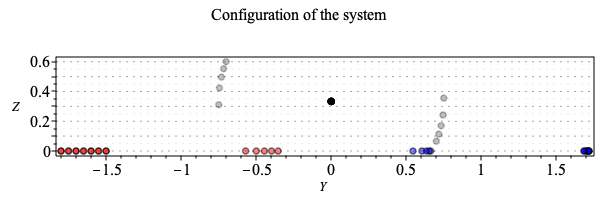
\includegraphics[scale=0.6]{images/Surge_conf.png}
  \caption{Plot of points, $q_{11}$, $q_{12}$, $q_{31}$, $q_{32}$ and end effector
  \label{fig:q11Configurations}}
\end{figure}

Figure \ref{fig:q11Configurations} is a plot of the how the points, $q_{12}$ (red), $q_{31}$(blue), $q_{32}$(blue), vary as the configuration of $q_{11}$ changes. From figure \ref{fig:q11Configurations}, the rotational the range of rotations for the platform can be computed. 

\begin{figure}[h!]
  \centering
  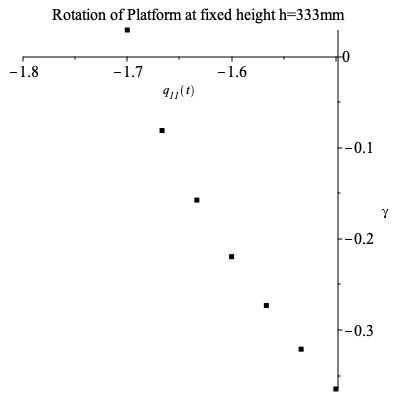
\includegraphics[scale=0.5]{images/Surge.png}
  \caption{Rotational angle of the platform at configuration $q_{11}(t)$
  \label{fig:angle}}
\end{figure}

At the fixed height of $33,3cm$ the platform has maximum unilateral rotation surge of approximately $20^{\circ}$. The solution is purely analytic because dimensions and limitations of the physical platform and joints are not considered. It is to say that a deeper position of the end effector yields a higher surge value, however is constraint by the platform edges hitting the ground. 

The total surge is therefore dependent on the platform width and height of the end effector position and constraint by the ground and the minimal distance between the slider 12 and 32.
It is also evident from Figure \ref{fig:angle} that initial displacements result in a higher gradient. This  could result in a loss in precision for small rotations. 

\begin{figure}[h!]
  \centering
  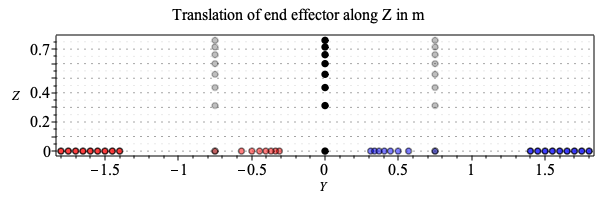
\includegraphics[scale=0.5]{images/Heave_conf.png}
  \caption{Plot of points, $q_{11}$, $q_{12}$, $q_{31}$, $q_{32}$ and end effector
  \label{fig:heave_conf}}
\end{figure}

\begin{figure}[h!]
  \centering
  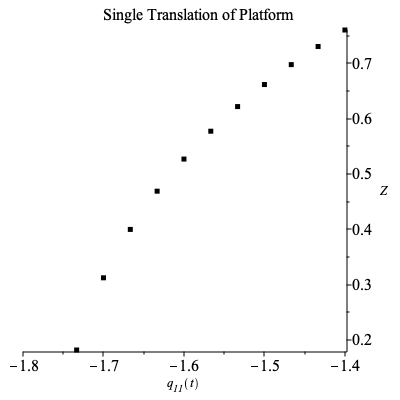
\includegraphics[scale=0.5]{images/Heave.png}
  \caption{Plot of points, $q_{11}$, $q_{12}$, $q_{31}$, $q_{32}$ and end effector
  \label{fig:heave}}
\end{figure}

Fixating the rotation of the system, as well as lateral translation results in 8 possible solution, using the above presented set up. Theoretically a range from $0$ to $750mm$ in heave is possible with the described setup. However physical constraints will make minimum and maximum positions less feasible. A reasonable range, regarding Figure \ref{fig:heave_conf} could be $400$ to $500mm$, according to the AB\,Dynamic brochure and a further benchmark review.

\subsection{Velocity Analysis}
Case A. Known velocity of independent coordinate.\newline
Case B. Known time law of independent coordinate.\newline


\begin{figure}[h]

\begin{subfigure}{0.5\textwidth}
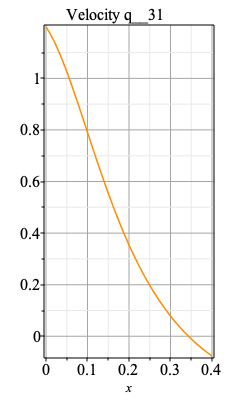
\includegraphics[height=0.9\linewidth]{images/Velocity31.png} 
\caption{Velocity of link 31}
\label{fig:subim1}
\end{subfigure}
\begin{subfigure}{0.5\textwidth}
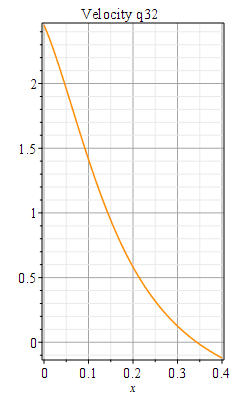
\includegraphics[height=0.9\linewidth]{images/velocity32.png}
\caption{Velocity of link 31}
\label{fig:subim2}
\end{subfigure}
\begin{subfigure}{0.5\textwidth}
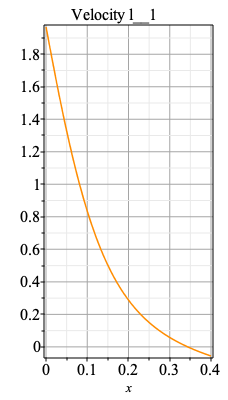
\includegraphics[height=0.9\linewidth]{images/Velocityl1.png}
\caption{Velocity of point 1 sliding in direction of link 12's inclination}
\label{fig:subim2}
\end{subfigure}\begin{subfigure}{0.5\textwidth}
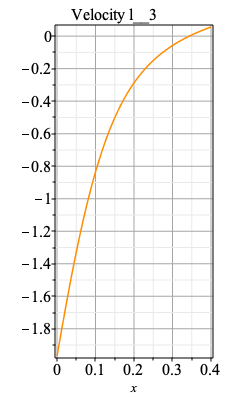
\includegraphics[height=0.9\linewidth]{images/Velocityl3.png}
\caption{Velocity of point 3 sliding in direction of link 32's inclination}
\label{fig:subim2}
\end{subfigure}
 
\caption{Caption for this figure with two images}
\label{fig:image2}
\end{figure}
   
\subsection{Acceleration Analysis}